\documentclass[12pt,a4paper,titlepage]{article}
\usepackage{graphicx}

\title{COP290: Design Practices\break\\User Registration App}
\author{Akshit Tyagi (2014EE10710) \\ Rishabh Kumar (2014PH10817) \\ Karan Dwivedi (2014CS10227) }
\date{15 January 2016}
\begin{document}
\maketitle

`User Registration App' is a simple Android app to test communication with a server using Volley JSON library. It takes in the names and entry numbers of team members through its user friendly GUI and sends it to the server when Submit button is pressed. We also check if the user types invalid (or blank) input.

The app also recieves the server response and shows it to the user. In case the server sent a ``Registration failed'' message, the app prompts the user to try again later.

The code for the project is being maintained in this repository:\\ {\em https://github.com/akshittyagi/AssignmentZero}.

\begin{figure}[!ht]
	\centering
	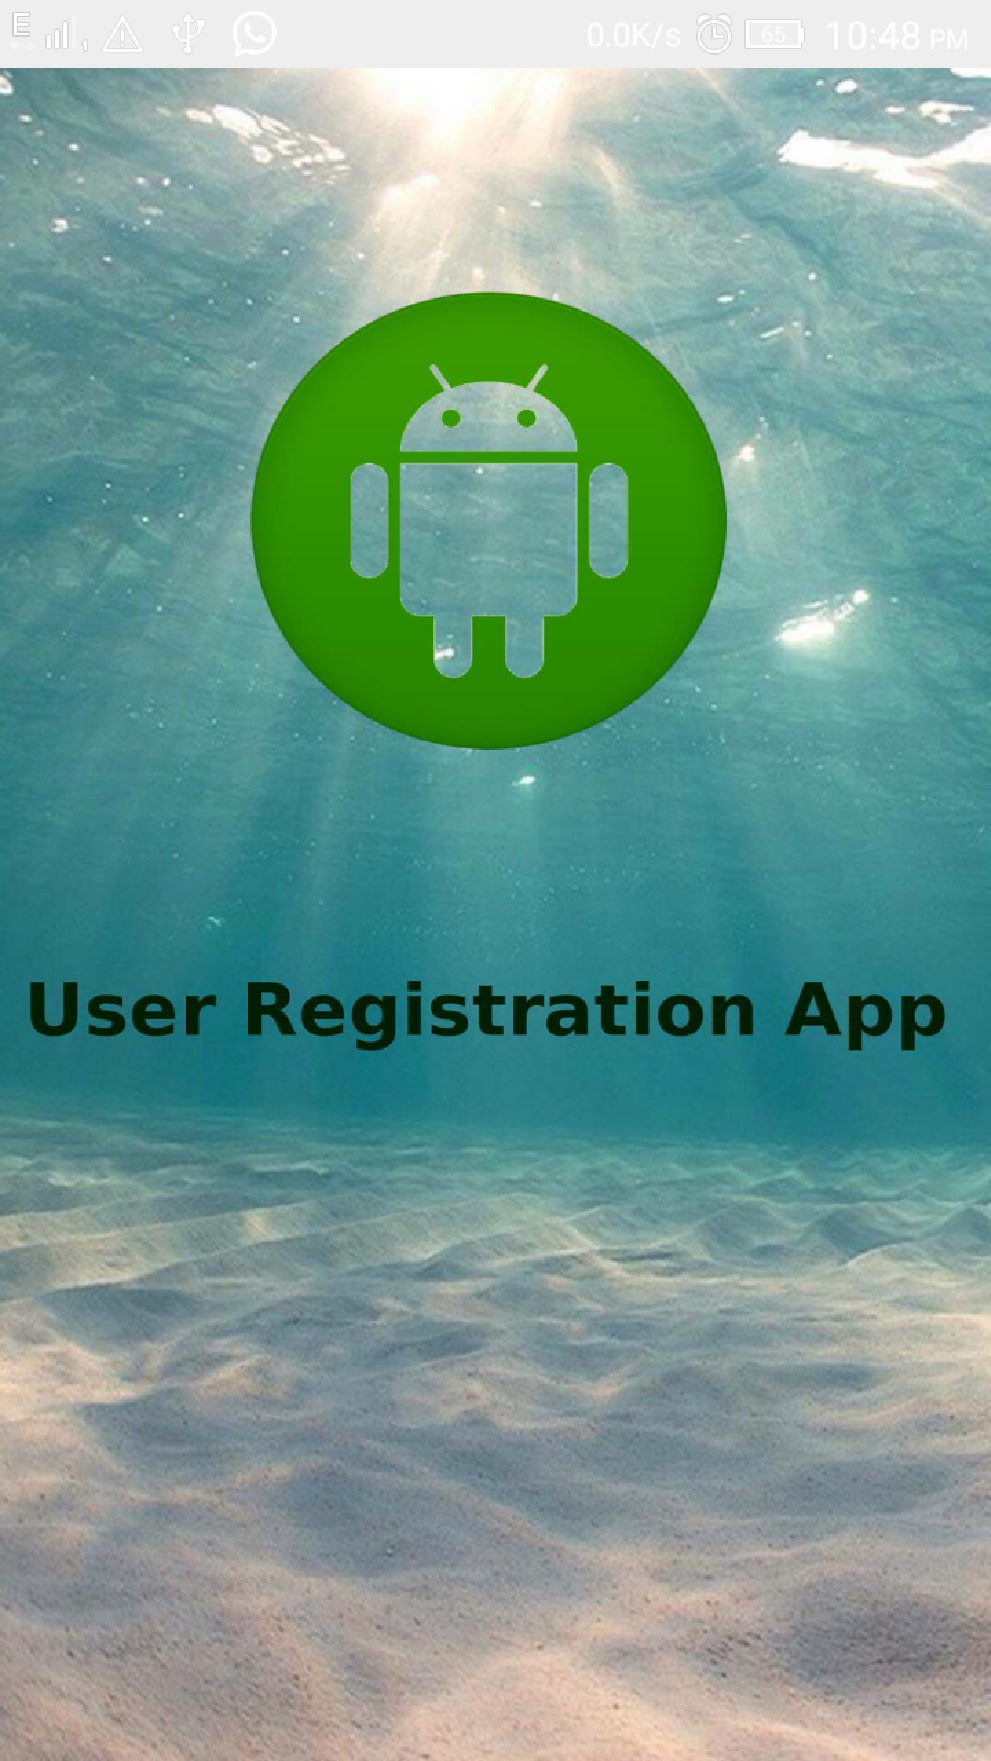
\includegraphics[width=0.5\textwidth]{./UserInterface}
	\caption{Splash Screen}
\end{figure}

\section{User Interface}

\begin{figure}[!ht]
	\centering
	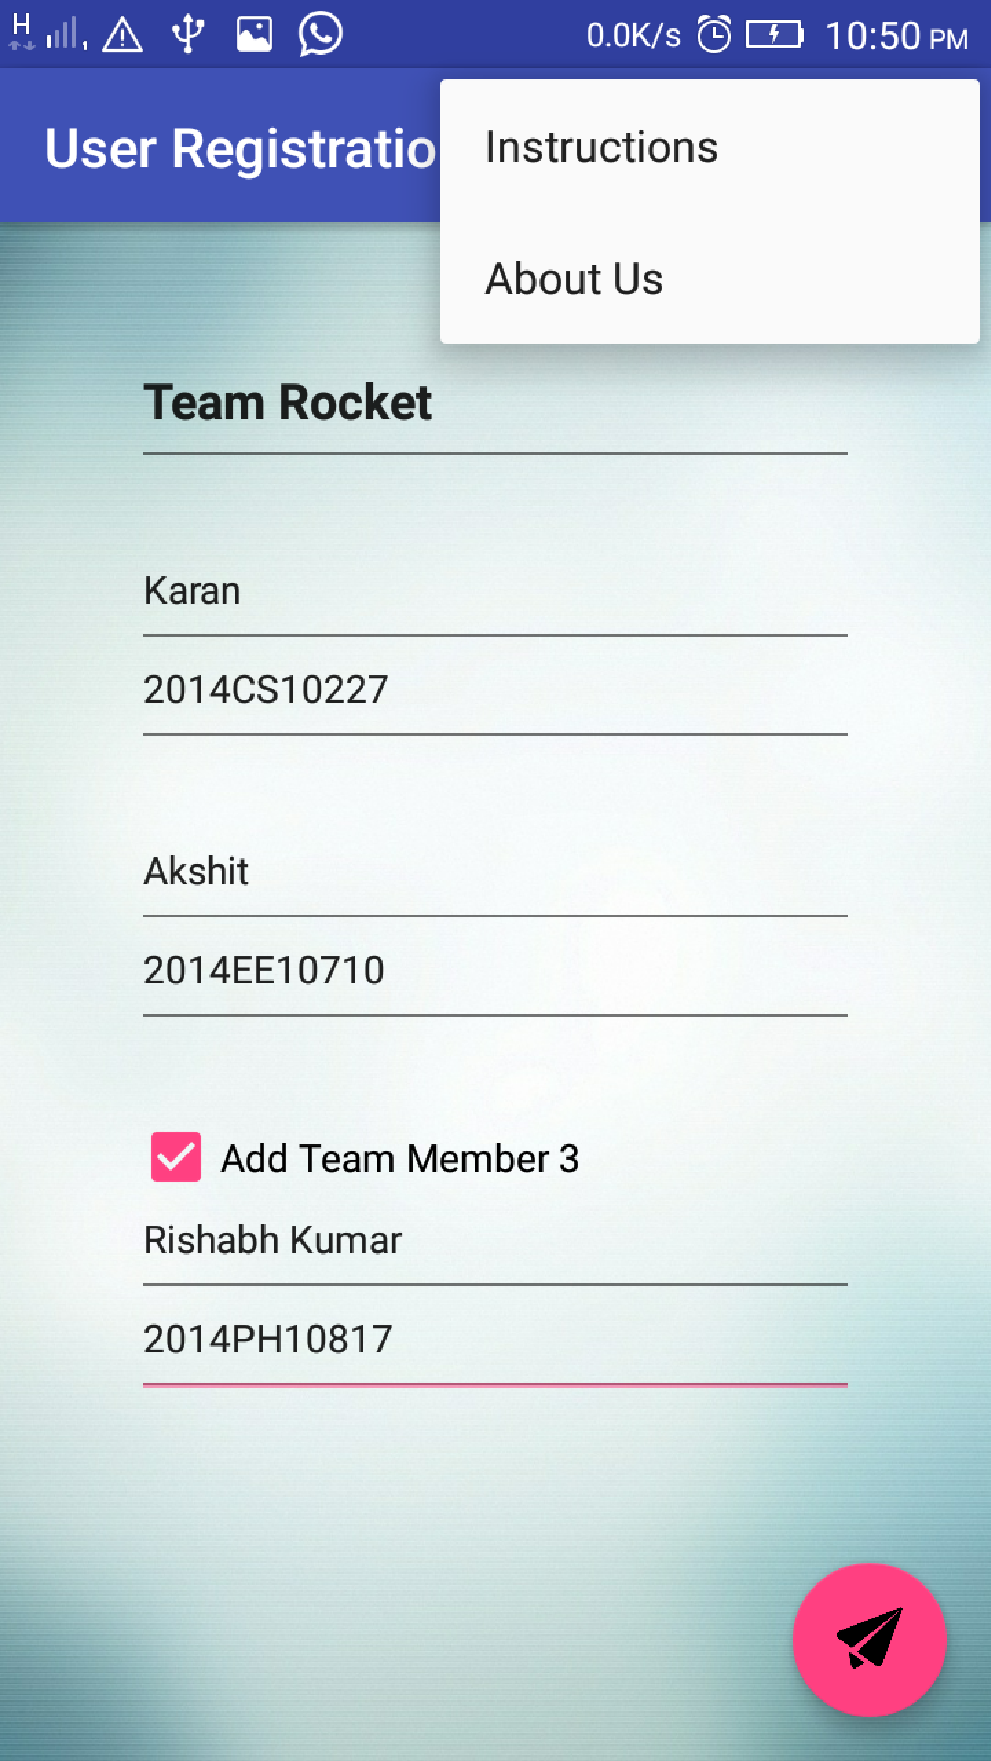
\includegraphics[width=0.5\textwidth]{./screen_main}
	\caption{User Input Screen}
\end{figure}
\begin{figure}[!ht]
	\centering
	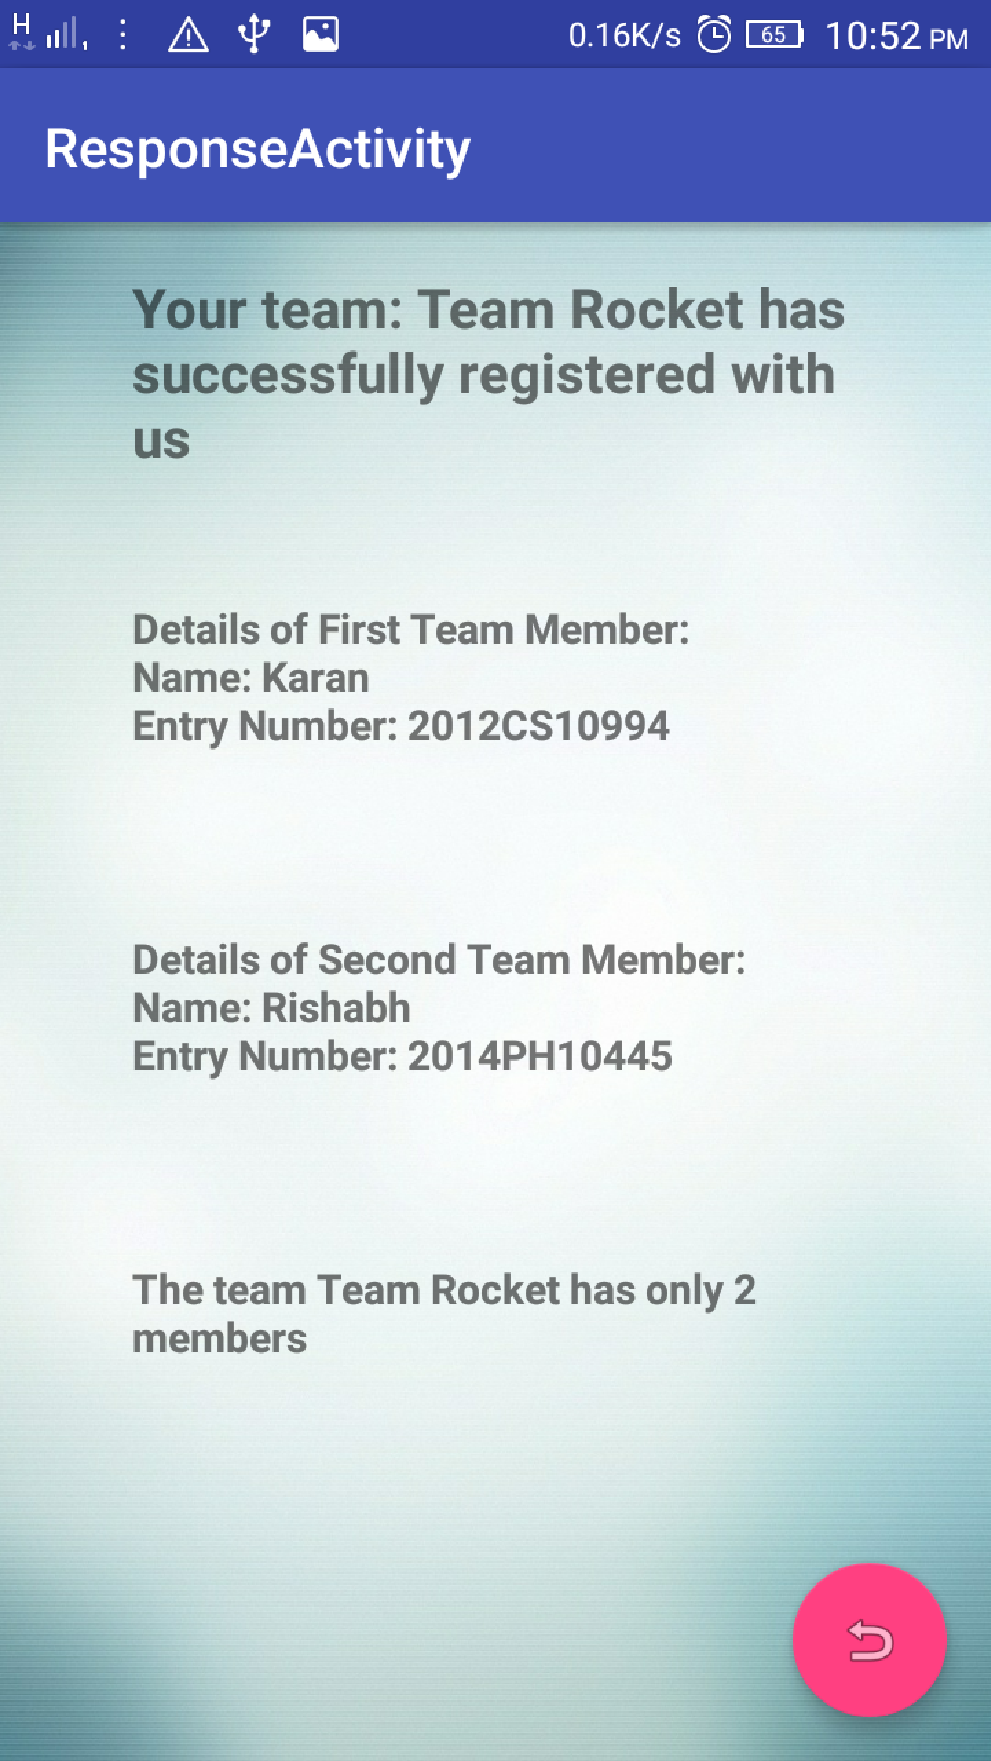
\includegraphics[width=0.5\textwidth]{./screen_response}
	\caption{Server Response Screen}
\end{figure}

\begin{itemize}
	\item \textbf{Details of the screens visible to the user}
	\item[] When the user starts the app, (s)he is greeted by the splash screen. Then the user sees a screen with input fields, where he can input his Team name and team members' details. The activity has 6 input fields and a floating action button. To register on the web server, the user enters the input using inbuilt keyboard and taps the submit button. In case there is an error in the input or the server response, the user is prompted to change it.
	      
	\item \textbf{Animations, buttons (enabled/ disabled under what conditions)}
	\item[] Following Google's material design principles, the screen has a floating submit button, which connects to the server only after the user has entered valid input in all fields. Otherwise, it highlights the incorrect inputs and prompts the user to correct them.
	\item[] When the Check Box `Team has 3 members' is checked, the third set of input fields becomes visible. On unchecking, it becomes invisible again.
	\item \textbf{Actions performed when a user enters information, presses a button/ icon etc.}
	\item[] When the user taps any input field, the keyboard shows.
	\item[] On pressing the submit button, the app checks the input and if found valid, sends it to the web server and recieves its response.
	\item[] This is shown to the user using a SnackBar on bottom of the page.
	\item[] The user can also read the instructions and know about the team through the Action Bar.
\end{itemize}

\section{Implementation Details}

\begin{itemize}
	\item \textbf{Organization of user information (Is it in a special User class, or is it distributed in arrays for each user entry)}
	\item[] Data is stored in a Java Map object.
	\item  High	level functions/methods used and descriptions of each one	
	\item [] checkValidity: Checks the validity of text entered on pressing the submit button.
	\item[] checkValidityName: Ensures name has only letters and is less than 16 characters long.
	\item[] checkValidityEntryNumber: Ensures Entry number follows the format used in IIT Delhi and only valid years, department codes are entered
	\item Methods for network communication.
	\item[] sendResult: Puts all data into a Map object and sends it using Volley RequestQueue object.
\end{itemize}


\section{Error Handling}
\label{error}

\begin{itemize}
	        
	\item Error Scenarios:
	\item[] An error is shown when the user enters invalid Entry Number or enters non characters in Name. The length of Name is restricted to 16 to avoid issues with server response.
	\item[] setError method is used to show a symbol and a help text to the user with relevant information.

\end{itemize}

\begin{figure}[!ht]
	\centering
	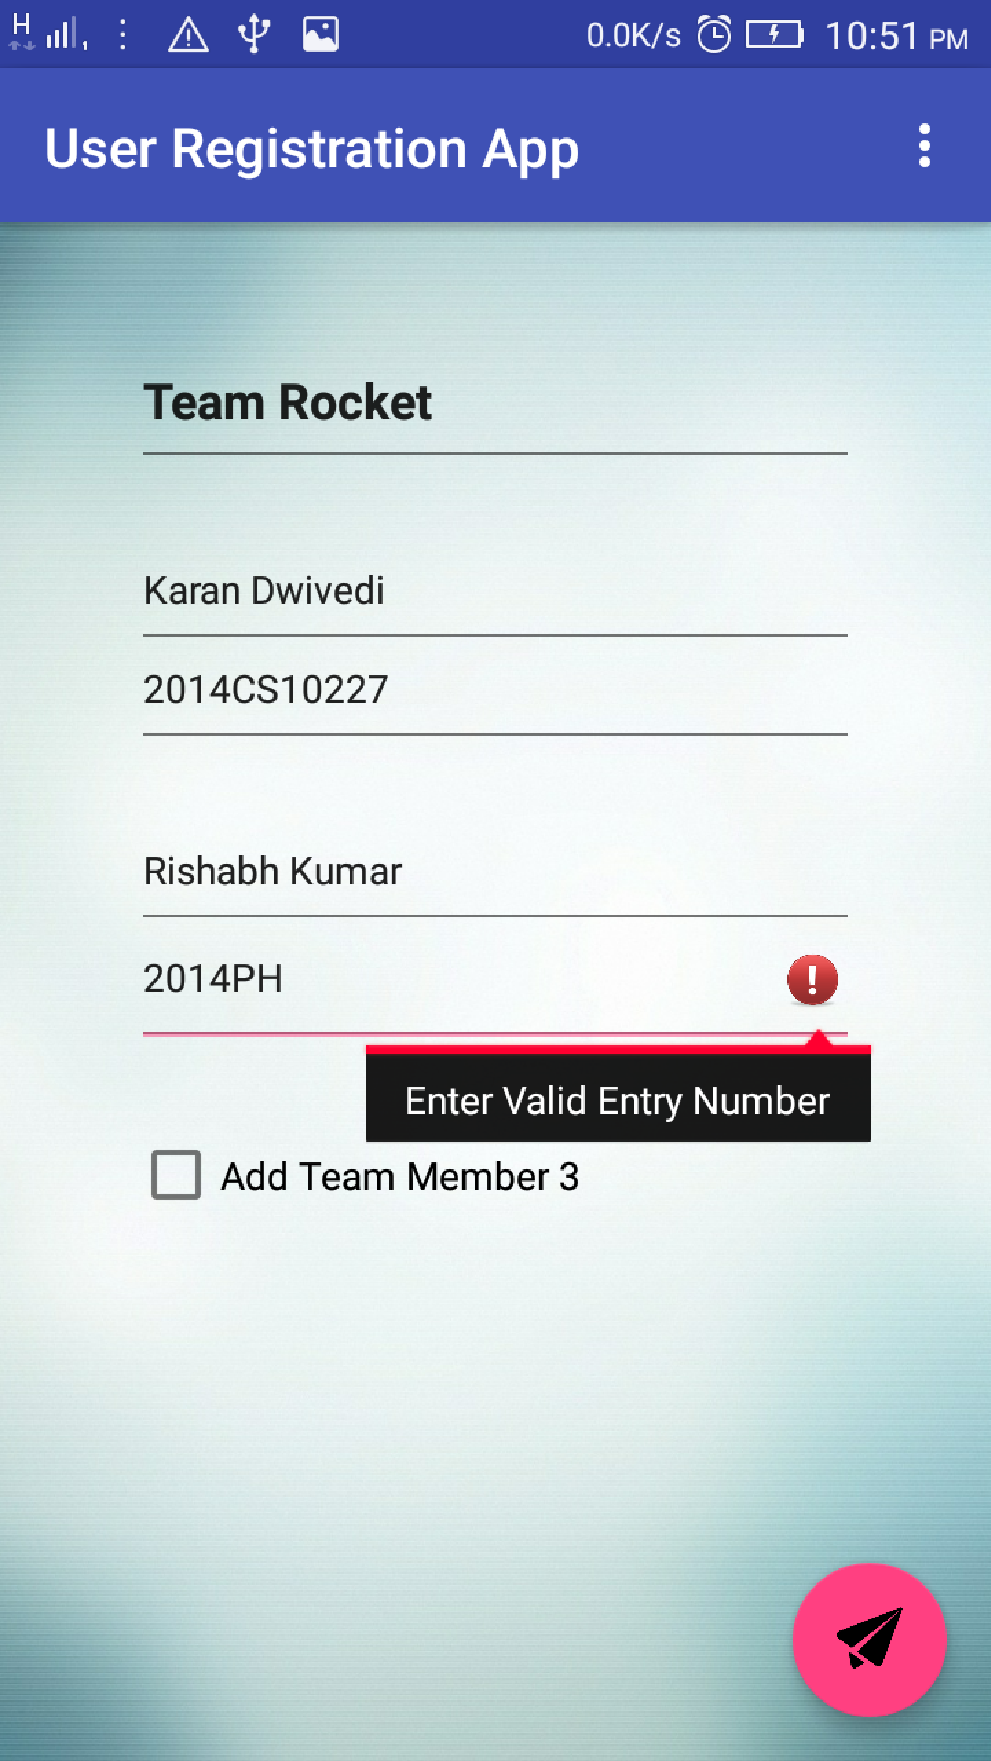
\includegraphics[width=0.5\textwidth]{./screen_error}
	\caption{Error Handling}
\end{figure}



\end{document}
